\documentclass[letterpaper, 10 pt, conference]{ieeeconf}  % Comment this line out
                                                          % if you need a4paper
%\documentclass[a4paper, 10pt, conference]{ieeeconf}      % Use this line for a4
                                                          % paper

\IEEEoverridecommandlockouts                              % This command is only
                                                          % needed if you want to
                                                          % use the \thanks command
\overrideIEEEmargins
% See the \addtolength command later in the file to balance the column lengths
% on the last page of the document

\usepackage[pdftex]{graphicx}
% TODO remember we need to meet color compliance:
% http://its.papercept.net/conferences/support/general.php

% TODO better name!
\title{\LARGE \bf
Approximately Orchestrated Road Traffic Automata\\
a General Traffic Simulation Framework
}

\author{Dustin Carlino, Mike Depinet, Piyush Khandelwal, and Peter Stone\\
        Department of Computer Science\\
        The University of Texas at Austin\\
        Austin, TX 78712\\
        {\tt \small\{dcarlino,msd775,piyushk,pstone\}@cs.utexas.edu}}

\long\def\commentp#1{{\bf **Peter: #1**}}
\long\def\commentpk#1{{\bf **Piyush: #1**}}
\long\def\commentm#1{{\bf **Mike: #1**}}
\long\def\commentd#1{{\bf **Dustin: #1**}}

%\long\def\commentp#1{}
%\long\def\commentpk#1{}
%\long\def\commentm#1{}
%\long\def\commentd#1{}

\begin{document}

\maketitle
\thispagestyle{empty}
\pagestyle{empty}

%%%%%%%%%%%%%%%%%%%%%%%%%%%%%%%%%%%%%%%%%%%%%%%%%%%%%%%%%%%%%%%%%%%%%%%%%%%%%%%%

\commentd{sounds fine to me, only thing is that we haven't actually focused on
  dynamic re-planning or any kind of overseer yet, although theres nothing
  stopping us from trying that idea again}
\commentp{If it's not implemented, we shouldn't talk about it.}

\begin{abstract} 
Autonomous vehicles have seen great advancements in recent years, and
such vehicles are now ever closer to being commercially available.
The advent of driver-less cars provides opportunities for optimizing
traffic in ways not possible before. This paper introduces an open
source multi-agent traffic simulator called AORTA, which stands for
\textit{Approximately Orchestrated Road Traffic Automata}, and
demonstrates its usage for optimizing autonomous traffic at a
city-wide scale. AORTA creates scale simulations by generating maps
using publicly available road data from \textit{OpenStreetMap}
(OSM). Simulations of specific regions throughout the world can be set
up in the few minutes it takes to export data for the region of
interest from OSM. AORTA focuses on interactions between agents by
defining \textit{behaviors} for individual vehicles and
intersections. These behaviors allow agents to interact with each
other as well as with an external \textit{overseer} that is
responsible for optimizing traffic flow. Overseers can interact with
these agents to allow for dynamic route re-planning to reduce traffic
load, optimized intersection navigation, and improved car following.
\commentpk{rest devoted to application}
\end{abstract}

%%%%%%%%%%%%%%%%%%%%%%%%%%%%%%%%%%%%%%%%%%%%%%%%%%%%%%%%%%%%%%%%%%%%%%%%%%%%%%%%

\section{INTRODUCTION}
\label{sec:introduction}

% theme: easy simulation in your city, in 2 minutes!
% be sure to emphasize open source!
% contribution: autonomous car / human car sim on EXISTING INFRASTRUCTURE

Autonomous vehicle technology has made tremendous progress in the last decade.
In 2004, the farthest distance traveled by a vehicle autonomously in the DARPA
Grand Challenge was $11.9km$ \cite{cnnGrandChallenge2004}. By 2007, six of the
competing teams completed the $96km$ course set for the DARPA Urban Challenge
\cite{spectrumUrbanChallenge2007}. They did so while following the same traffic
laws followed by human drivers, navigating along with other moving vehicles,
and following correct intersection precedence order. Since then, Google's
driver-less cars have clocked more than $250,000km$ on public roads in urban
California, USA \cite{tedThrun2011}. In 2010, researchers from the University
of Parma successfully completed an autonomous \textit{intercontinental} run
from Parma, Italy to Shanghai, China \cite{cnnVislab2010}. The successful
completion of all these milestones suggests that autonomous cars are here to
stay, and are ever closer to becoming commercially available. 

The arrival of driver-less cars presents several challenges that need to be
addressed in the near term. Road infrastructure needs to be updated to better
support autonomous vehicles.\commentp{Is this necessarily the case?
  It may be useful, but is it a need?} A number of legal and safety concerns need to be
addressed in the context of driver-less cars. Human drivers need new
methodologies to interact with autonomous drivers on public roads. At the same
time, driver-less cars provide opportunities of solving traffic problems in
ways that were never before possible. For instance, autonomous cars can be
quickly diverted to make way for emergency vehicles responding to an accident.
Even day-to-day traffic issues such as congestion could potentially be greatly
reduced by effective management of traffic flow. This work addresses
some of these problems.\commentp{Be more specific in this paragraph.
  Which of these challenges are eing addressed elsewhere (cite), and
  which are addressed in this paper?}
\commentp{Overall, this paragraph is a bit scattered.  I suggest
  something more like the following (after the first sentence).
  Several of the challenges are already being addressed.  For example
  .....
  This paper focusses on the specific challenge(s) of....}

\commentd{nevada even made autonomous cars legal:
http://www.pcmag.com/article2/0,2817,2400400,00.asp}

\commentd{another example long-term usage: fuel. I went to a talk by
  somebody on the engr side about powermiling and optimizing battery usage}

\commentd{we don't support lane-changing yet, and overseers arent re-implemented
yet either}

\commentp{legal issues are addressed here:  http://www.path.berkeley.edu/PATH/Publications/PDF/PRR/2009/PRR-2009-28.pdf}

\begin{figure}[h]
  \centering 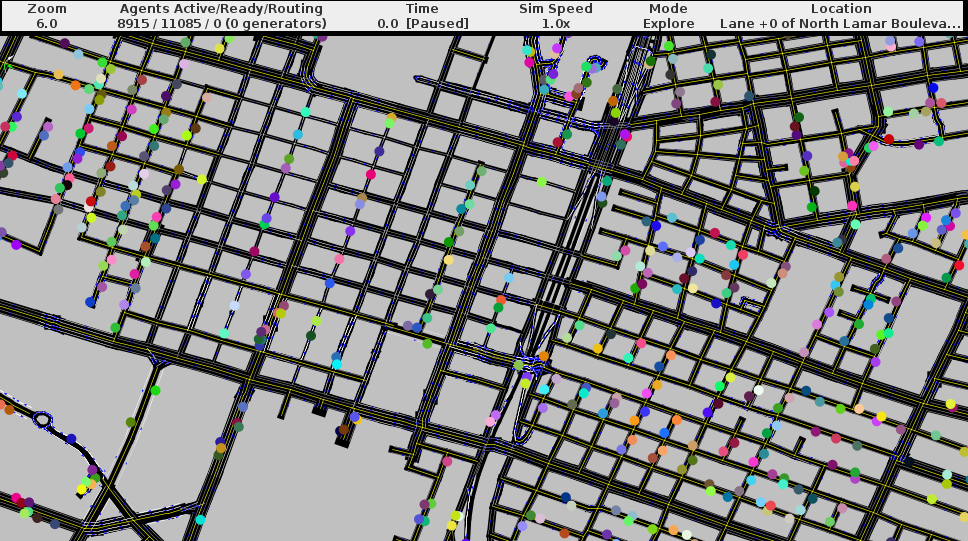
\includegraphics[width=\linewidth]{downtown_atx.png}
  \caption{A simulation of downtown Austin, Texas.}
  \label{fig:ui_screenshot}
  \vspace{-10pt}
\end{figure}

% TODO reference the screenshot

This paper introduces an open source multi-agent microscopic traffic
simulator called AORTA, which stands for \textit{Approximately
Orchestrated Road Traffic Automata}. The AORTA simulator focuses on
the interactions between individual vehicles and intersections, both
of which act as \textit{agents} in AORTA's framework. Vehicles
interact with other vehicles to pass and change lanes, and interact
with intersections to decide when to cross them. Researchers
developing applications on top of the AORTA simulator define
\textit{behaviors} that these agents follow to interact with one
another. To optimize traffic flow, external \textit{overseers} can
coordinate with these agents to provide recommendations such as route
suggestions or intersection signaling policies.  An advantage of such
an approach is that by assigning human-like behaviors such as the
``car following model'' \cite{brackstone1999car} to vehicles, and
traffic-signal-like policies to intersection, AORTA can just as easily
simulate human traffic.

Like any other microscopic traffic simulator, AORTA needs maps to run
simulations. One of AORTA's key features is that it generates maps using road data available from OpenStreetMap
(OSM) \cite{osm}, a Wikipedia-like interface for world maps. Researchers using
AORTA can export any relevant map area from OSM. This map is then parsed by AORTA to
create scale simulations of the real world. A researcher employing AORTA can have a simulation
of any part of the world for which OSM has data running in about five minutes
(allowing for download time).  AORTA also has the advantage of being open source and
easy to install so that researchers can make any tweaks they find necessary.
\footnote{http://code.google.com/p/road-rage}

\commentpk{Needs 1 more para based on final application}

% Section 2 will review other traffic simulators. Section 3 will introduce the
% overall architecture of AORTA. Section 4 describes how OSM maps are used.
% Section 5 explains the simulation engine and the properties AORTA posses that
% are useful for general traffic experiments. Section 6 gives some initial
% results from such an experiment, and Section 7 concludes.

%%%%%%%%%%%%%%%%%%%%%%%%%%%%%%%%%%%%%%%%%%%%%%%%%%%%%%%%%%%%%%%%%%%%%%%%%%%%%%%%

\section{RELATED WORK}
\label{sec:related_work}

% just draw differences between us and them

Computational processing power has made excellent advancements in the
last two decades. Parallel computing has proved significant for
traffic simulation through the use of Geographic Information System
(GIS) software \cite{pursula1999simulation}. Advanced computing
techniques have enabled microscopic models of traffic simulation to
generate results at a meaningful scale (city-wide or greater). As a
result, a number of good micro-simulators have been introduced in the
past decade. We review a number of such simulators in this section
along with other relevant work.

A number of traffic simulators already make use of OSM data. MATSim is one such
multiagent simulator that focuses on performing large-scale simulations in a
relatively small amount of time \cite{balmer2009matsim}. Traffic demand is
supplied to MATSim in the form of \textit{plans} that an individual may intend
to follow in a given day. MATSim aims to iteratively improve these plans though
offline computation to maximize traffic throughput. In other words, it helps
individuals understand the best way to go about their daily routine to minimize
time spent in transit. This goal is somewhat different from that of AORTA,
where the demand supplied by individuals is taken as is. Instead, AORTA aims to
reduce traffic congestion through interactions with individuals in real-time
based on the current demand.

\commentd{last sentence above... we're not not doing that yet, and we dont
  discuss it further here.}

Another popular open source traffic simulator that can use OSM data is SUMO
\cite{SUMO2011}, which shares the same goals as AORTA and is fairly similar at
a high level. SUMO has been used to study the effect of automated
transportation systems, route planning of individual vehicles, as well as
dynamically adapting traffic signal policies to increase traffic efficiency.
AORTA and SUMO differ in the manner in which intersections are handled. SUMO
uses traditional traffic signals, while AORTA adopts a much more general
\textit{reservation} system. A reservation tells a car when it is safe to take
its desired path through the intersection. Reservations can be allotted to
vehicles through more traditional means such as traffic signals or stop-sign
based intersection precedence, or through more efficient methods designed
specifically for autonomous vehicles \cite{JAIR08-dresner}.
%\commentpk{does the above difference seem a bit pedantic?}  

On the other hand, there are a number of simulators that specifically
target autonomous traffic systems. One such system is AIM
\cite{JAIR08-dresner}, which aims to optimize traffic flow between
autonomous vehicles at a given intersection. AIM studies problems at
the scale of roughly a dozen intersections arranged in a regular grid,
while AORTA has the potential to apply some of the same research at a
city-wide scale to real-world road networks. A few simulators focus on
autonomous vehicles with sensors and actuators
\cite{figueiredo2009approach}. These simulators are used to ensure
that autonomous vehicles are behaving correctly while interacting with
other vehicles and infrastructure. On the other hand, AORTA assumes
that autonomous vehicles are capable of reasonable driving, and
focuses on interactions between agents to optimize traffic flow.

Autonomous agents have also been used in the past to model human
traffic. For instance, one approach models human merging and lane
changing behavior through the use of autonomous agents interacting
with one another \cite{hidas2002modelling}. Another approach attempted
to improve traffic congestion for human drivers by using a network of
autonomous intersections.  These intersections have the ability to
interact with one another and execute a dynamic traffic signal policy
minimizing overall wait time \cite{manikonda2001autonomous}.

\commentd{and we can do the above too. we talk about how to make the current
  behavior more flawed and humanlike in the agent reactions section.}

%%%%%%%%%%%%%%%%%%%%%%%%%%%%%%%%%%%%%%%%%%%%%%%%%%%%%%%%%%%%%%%%%%%%%%%%%%%%%%%%

\section{ARCHITECTURE}
\label{sec:arch}

% Diagram made with gliffy.com. architecture.gxml should enable editing.
\begin{figure}
  \centering 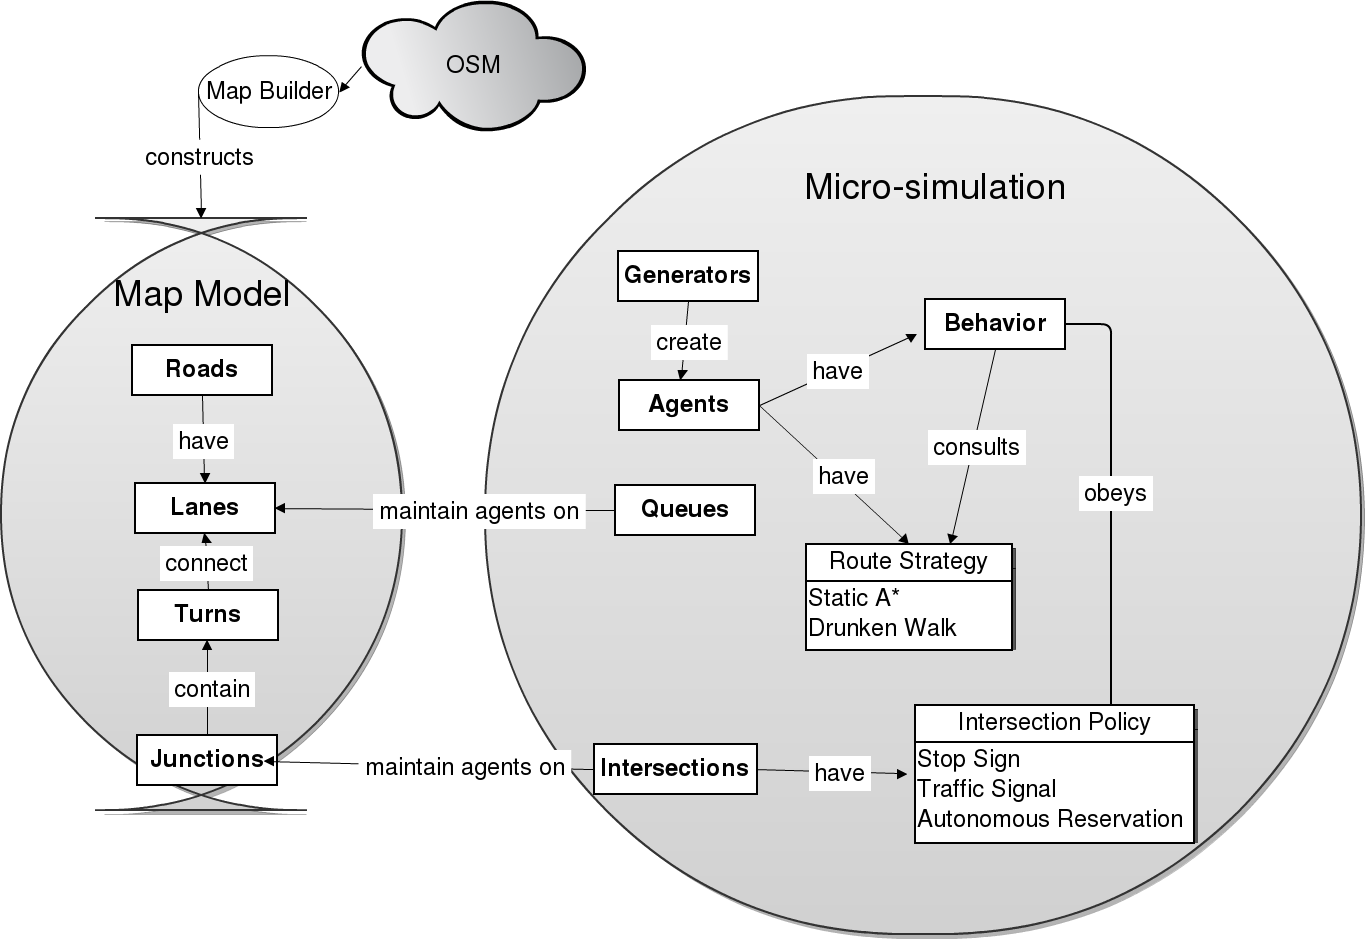
\includegraphics[scale=0.3]{architecture.png}
  \caption{A summary of AORTA's components.}
  \label{fig:arch}
  \vspace{-20pt}
\end{figure}

AORTA is divided into three modular components: the map model, micro-simulation
engine, and user interface (UI). The map model transforms OSM maps into AORTA graphs, then
answers pathfinding and geometry queries. The simulation engine adds a notion of
agents, vehicle dynamics, and collisions. Finally, the UI can
interactively render the map and agents. A headless mode also enables running
experiments without the overhead of visualization. The interaction between
modules is visualized in figure \ref{fig:arch}.

AORTA's implementation uses Scala, a language implemented on the Java Virtual
Machine \cite{scala}. Scala provides the advantage of functional programming
constructs while still permitting imperative style.  Extensions and clients
built on top of AORTA can be written in either Java or Scala. The software is
open-source \footnote{source code at http://code.google.com/p/road-rage} and
easily extensible. For instance, the stop sign sign policy used in experiments
described in section \ref{sec:results} is implemented in just 70 lines of code.

%%%%%%%%%%%%%%%%%%%%%%%%%%%%%%%%%%%%%%%%%%%%%%%%%%%%%%%%%%%%%%%%%%%%%%%%%%%%%%%%

\section{MAP CONSTRUCTION FROM OSM}
\label{sec:map}

One advantage of AORTA is that it simulates traffic on existing infrastructure
rather than randomly generated maps. Utilizing OpenStreetMap \cite{osm}, a
community project offering user-editable, free XML-based maps, enables this. To
run a simulation on a map from OSM, there is a one-time conversion process to
transform the map into AORTA's format, which encodes information about lanes and
turns not contained in the OSM source.

\subsection{Map Model}

%\pix{map_model.png}
%    {Roads contain several lanes, and intersections contain several turns
%     between lanes.}
%    {scale=0.5}

A map is represented as a directed graph with \emph{lanes} as edges and
\emph{turns} as vertices. A \emph{road} groups one or two sets of lanes
together, one set for each direction of travel.
\emph{Intersections} map the possible turns from incoming to outgoing lanes.
Since both lanes and turns support traffic, they are grouped together as
\emph{traversables}, meaning agents may exist on them.

The map also has a geometric interpretation, used for visualization and
measuring physical distances. A road contains a sequence of points, defining the
center line that divides the road into two directions of travel. AORTA
interprets these points as straight lines and projects parallel lanes out using
a fixed width. Turns are modeled with a single straight line connecting the end
of one lane to the start of another (so right turns often have 0 length).

\subsection{Map Construction Passes}

The builder works by incrementally transforming OSM graphs into AORTA graphs,
with each pass feeding the next.
\begin{enumerate}
  \item OSM encodes many paths besides driveable roads, so the builder first filters
        these out. Next the builder marks GPS nodes common to multiple roads, since
        they implicitly indicate intersections. Overpasses do not share nodes
        with the roads they cross \cite{osmOverpass}.
  \item OSM \emph{ways} (sequences of GPS locations) include many
        intersections, so the builder next splits ways into undirected
        segments of roads between exactly two intersections.
  \item The builder multiplies undirected roads into directed lanes in each
        direction (unless the road is marked one-way). The builder guesses the
        number of lanes based on OSM's ``road type'' tag or an explicit number of
        lanes, when that data is available.
  \item The builder constructs turns between incoming and outgoing lanes at each
        intersection. The angle between the two lanes determines whether the turn is
        a left, right, straight, or U-turn. When several lanes all cross into fewer
        lanes, the builder forces merging of the rightmost lanes. Although
        inaccurate, these patterns are the best compromise with the available data.
  \item Because turns are heuristically placed, the graph is often disconnected.
        In order to ensure that an agent will be able to reach any point in the map,
        the builder removes all but the largest strongly connected component of the
        digraph.  Disconnected lanes are spliced out of larger roads, leaving
        unappealing geometric gaps, but correctly ensuring connectivity for
        corner-case free pathfinding.
  \item The builder serializes the graph in a simple XML format.
\end{enumerate}

%%%%%%%%%%%%%%%%%%%%%%%%%%%%%%%%%%%%%%%%%%%%%%%%%%%%%%%%%%%%%%%%%%%%%%%%%%%%%%%%

\section{SIMULATION}
\label{sec:simulation}

AORTA uses microscopic simulation, modeling individual drivers as agents.
Time is modeled discretely, meaning an agent accelerates at a fixed rate for
the duration of a ``step'' to achieve a new position and velocity. Space is
continuous, meaning agents occupy a moving interval of a lane, rather than one
fixed tile of the road. Each step lasts the same fixed duration \textit{dt}.
This lets agents reason about how far they will travel for a given choice of
acceleration before being able to choose a different acceleration. Setting
\textit{dt} to the ``reaction time'' of a human driver may be appropriate for
experiments modeling humans.

Currently agents cannot switch lanes. AORTA allows merging lanes by treating
the merge point as an intersection. \commentpk{i take it this is an orphan
paragraph?} \commentd{yeah, where should it belong?}

Each step, the simulation does the following:

\begin{enumerate}
  \item Introduces new agents into the map
  \item Updates the position and velocity of agents based on their choice of
        acceleration in the previous step
  \item Checks for collisions
  \item Allows each agent's behavior to choose an action for the next step
\end{enumerate}

Each step (except 2) will be described below, followed by limitations of the
simulator. Section \ref{sec:config} will describe how researchers may easily
modify relevant portions of AORTA.

\subsection{Spawning new agents}

To introduce new agents into the simulation in real-time, users can create
\emph{generators} programatically or using the UI. The generator produces the
desired amount of traffic by initializing agents from random locations inside a
\textit{start} polygon to random destinations within a \textit{goal} polygon.
Users can draw these polyons by mouse in the UI, allowing specific traffic
patterns like rush-hour scenarios to be easily simulated. A generator polygon
may also cover the entire map, uniformly distributing traffic everywhere.

Every step, a generator creates some number of new agents. If the agent's route
policy needs computation like pathfinding to operate, the generator either
performs it immediately (incurring a delay in simulation if it is running) or,
if possible, sends it to a pool of worker threads to process in the background.

Once an agent's route is ready, the agent waits alongside its starting lane (as
if it is in a driveway or parking lot). When the lane has no agents that could
potentially crash with the new vehicle, the new agent enters the system with
zero initial speed. Because behaviors must enforce speed limit along a lane
from the moment an agent enters a road, it is safe for a new agent to enter a
road if there is no other agent within the worst-case distance (traveling
distance at the speed limit, plus stopping distance from this speed) preceeding
the spawn point.% To avoid predicting which agents might enter the lane in the
%near future, there is a buffer space at the beginning of the lane where a new
%agent may never spawn. This disqualifies some short lanes from being spawn
%points, but this is not a big limitation in practice. \commentpk{I understand
%your concern about explaining the entire methodology, but the last 2 lines are
%unnecessary and somewhat distracting}

\subsection{Collision checking}

All traversables (lanes and the straight line-approximation of turns) maintain
an ordered queue of occupying agents. One simulation step happens atomically,
meaning collision checking occurs after all agents have moved. If this were not
the case, false positives could occur when an agent steps before the agent in front
of it. A collision is defined as the reversal of order of agents during a step.

Likewise, intersections check for collisions by examining the turn each agent is
performing and verifying that no other agent is simultaneously performing a
conflicting turn. AORTA has a low-granularity model of turn conflict. If two
vehicles at any point along two different turns could ever come into contact,
then the turns are always in conflict, no matter where the agents actually are
along that turn. This is visualized in figure \ref{fig:conflicts}. The
alternative of tiling intersections \cite{JAIR08-dresner} would provide more
granularity, but it adds computational complexity and would be impractical for
many of the complex intersection geometries inferred from OSM.

When a collision occurs, the simulator throws warnings and halts, since this
indicates a bug in some policy. A future alternative could be to mark the region
as impassable and re-route other traffic away from the accident.

\begin{figure}[h]
  \centering 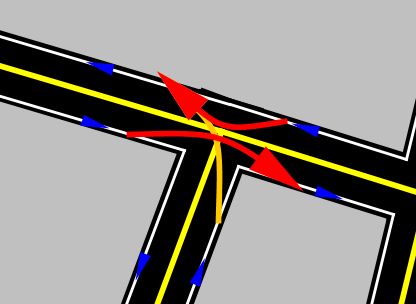
\includegraphics[scale=0.5]{turn_conflicts.png}
  \caption{An agent cannot turn left while agents on the perpendicular road cross}
  \label{fig:conflicts}
  \vspace{-15pt}
\end{figure}

\subsection{Agent Behavior}
\label{sec:behaviors}

Each agent has a \emph{behavior} governing it, responsible for obeying
intersection policies and avoiding collisions. When the agent travels past the
end of a lane during its step, the behavior picks the turn to take. At each
step, the behavior can make the agent react by performing one of two actions:
disappearing from the map (when the agent is at rest and is done with its route)
or setting an acceleration for the next step. Were lane changing modeled, that
would be another possible action.

Currently, all agents use a primary behavior that is a generalized, baseline
behavior that guarantees not to collide with another agent or enter an
intersection at the wrong time. Since it picks the highest safe choice of
acceleration at each step, it could easily be extended to mimic human drivers by
traveling at some random lesser acceleration or to optimize fuel efficiency
by tuning movement.

The default behavior maximizes acceleration while obeying speed limits,
avoiding collisions, and obeying intersections. By considering the highest speed
achievable at the end of the next step and the subsequent stopping distance at
this speed, the behavior's lookahead engine can scan sufficiently far ahead
along several traversables to locate agents to avoid and intersections to query.
The analysis short-circuits at the first nearby agent and intersection requiring
a stop, since it would be illegal to drive further anyway.

\subsection{Simulation Limitations: Gridlock}

Agents maintain a safe following distance from the next agent. If a lane is
filled, then an agent may be forced to stop in an intersection mid-turn and
block other traffic. The default behavior prevents this by refusing to start a
turn before the lookahead engine guarantees no agent will trigger a premature
stop.

However, with very high volumes of traffic, it is possible for waiting agents to
accumulate and fill lanes to their capacity. When this happens in a circular
manner so that the agent at the front of each lane is waiting to perform a turn
into another full lane with the same such head agent, gridlock \cite{gridlock}
occurs; no agent in the system will make progress unless an agent at the front
decides to pick a different turn. Figure \ref{fig:gridlock} demonstrates this.
AORTA can detect this by finding cycles in the graph of the ``is following''
relation.

\begin{figure}[h]
  \centering 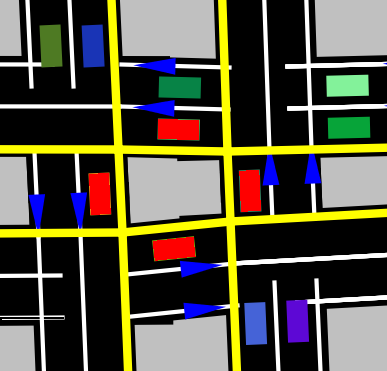
\includegraphics[scale=0.25]{gridlock.png}
  \caption{Each of the red agents wants to turn left, so none of them
           can. The traffic jam will slowly build up around this intersection.}
  \label{fig:gridlock}
  \vspace{-10pt}
\end{figure}

In many observed cases, the gridlock is caused by AORTA's present lack of
lane-changing support: agents loop around these intersections in order to enter
a lane adjacent to their original lane. Since these routes are still legal, it
is desirable to prevent or mend this without forcing different routes. The
conditions under which every vehicle eventually may proceed are known.
\cite{AAAI11-au}.

%%%%%%%%%%%%%%%%%%%%%%%%%%%%%%%%%%%%%%%%%%%%%%%%%%%%%%%%%%%%%%%%%%%%%%%%%%%%%%%%

\section{CONFIGURABILITY}
\label{sec:config}

There are three main components of the simulation, each configurable by
extending built-in implementations of an interface: agent behaviors, routing
strategies, and intersection policies. Behaviors have been described already in
section \ref{sec:behaviors}.

\subsection{Intersection Policies}

A behavior's interaction with an intersection policy amounts to polling it with
the turn the agent wants to perform, the distance away the agent currently is,
and how long the agent has been waiting (so policies can enforce a required
delay before entering the intersection). The intersection policy simply orders
the agent to ``stop'' or ``proceed.'' The acceleration chosen to avoid entering
an intersection attempts to account for crosswalks by ending a configurable
threshold before the end of a traversable.

Intersection policies are one of the most intriguing aspects of the simulation
to tweak, especially in light of autonomous vehicles. Current policies include
traditional stop signs, traffic signals, and an AIM-inspired autonomous
reservation system \cite{JAIR08-dresner}. The traffic signals are further
extensible by assigning groups of non-conflicting turns at each intersection
with some duration and offset. The experiment in section \ref{sec:results}
features standard turn grouping (turns from parallel incoming directions are
scheduled simultaneously, and left turns are grouped) and a breadth-first search
heuristic for propagating timings. Future policies could include signals that
adapt timings and refinements to the autonomous reservation policy.

\subsection{Routing Strategies}

Picking accelerations that optimize objective functions is a separate task from
picking a path to travel. Agent behaviors consult a route strategy to pick
turns. Currently two simple implementations are available. One statically plans
a route to some goal using standard A* search \cite{astar}. The other performs a
drunken walk, lazily planning random choices at each intersection as the
lookahead engine requires, choosing the direction that minimizes the Euclidean
distance to the goal with 75\% probability. Researchers can experiment with
dynamic replanning or hierarchial planning without modifying any code other than
creating a new route implementation. Route policies could also interact with a
singleton overseer to gain some sort of global insight or with smart
intersections to avoid congestion.

%%%%%%%%%%%%%%%%%%%%%%%%%%%%%%%%%%%%%%%%%%%%%%%%%%%%%%%%%%%%%%%%%%%%%%%%%%%%%%%%

\section{EXPERIMENTAL RESULTS}
\label{sec:results}

A particular focus of AORTA is intersection policies. To demonstrate how much
policy affects agent performance, three policies are evaluated: stop sign,
traffic signal, and autonomous reservation. These are compared with all other
parameters fixed:

\begin{enumerate}
  \item the map (a 6 by 7 mile slice of downtown Austin, Texas
        \footnote{bounded by the Mopac and Springdale Road horizontally,
        and Oltorf Street and Koenig Lane vertically})
  \item dt = 0.1 seconds
  \item the agents spawned and their routes -- a continuous generator creates
        one new agent every 1 simulation second, with a uniformly random
        starting position and goal
  \item the duration of the experiment: one hour
\end{enumerate}

Each experiment is deterministically reproducible. A seed for the pseudo-random
number generator, the input graph, and the generators' configuration fully
determine the outcome of any simulation \footnote{This determinism may break
  down when generators use worker threads, since routes may be computed in
different orders, causing agents to enter the road at different times.}. After
setting up a scenario in the UI, users can save this configuration for
resimulation.

The speed of simulation depends on the step duration dt, the map size, and the
number of agents. A measure independent of these factors is the number of agent
steps per second. On a 2.4 GHz machine, this can be observed to average at about
150,000, a number comparable to existing simulators \cite{SUMOthesis}. When dt
= 0.1 seconds, this means 15,000 agents can be comfortably simulated in
real-time. Further optimizations are planned.

\subsection{Experiment parameters}

Each policy has parameters, so the configuration used is relevant. Stop signs
accept agents FCFS, refusing agents until they have idled at 0 speed for 1
second. This delay approximates human reaction time. The traffic signal policy
requires timings and groups of simultaneous turns for each intersection. The
configuration tested here uses a breadth-first search from one major road's
lanes to try to synchronize green signals for the agents near that lane to not
stop for several intersections. This heuristic needs improvement in how it
handles the remaining groups of turns that are scheduled after the first
sequence. Finally, the autonomous reservation policy allows new agents to join
existing groups of agents if their turn is compatible with the others. To
prevent one heavy direction of traffic from hogging the intersection
indefinitely, a timeout preemptively cycles through reservations. Ideally this
should be based on the relative numbers of agents depending on their
group of reservations.

\subsection{Results}

\begin{figure}[h]
  \centering 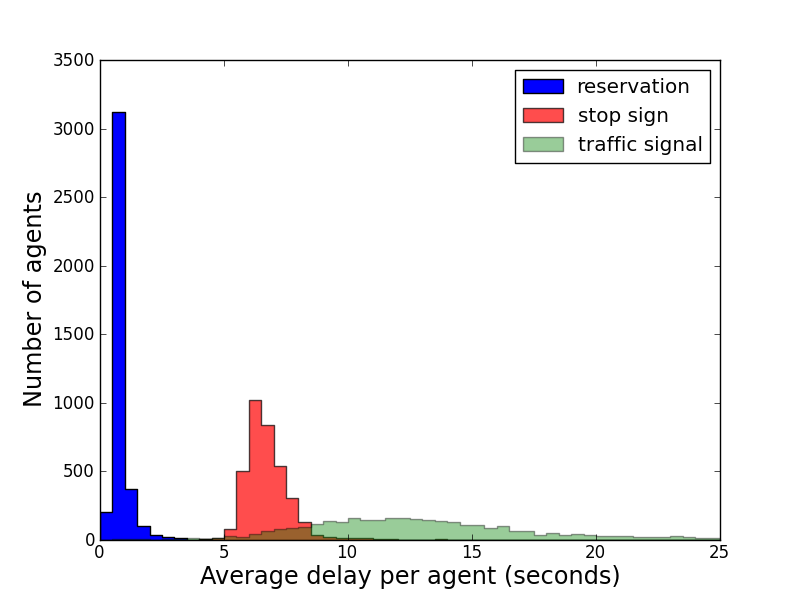
\includegraphics[width=\linewidth]{avg_lag_agent_atx.png}
  \caption{The distribution of average delay reveals that traffic signals can
           cause the most lag.}
  \label{fig:avg_lag}
  \vspace{-10pt}
\end{figure}

If an intersection immediately permits an agent to proceed and grants other
agents in the same lane similar access (because this new agent must still follow
these others), then the new agent may simply proceed at full speed limit without
pausing. This gives the least possible delay spent along some lane, so any extra
time is defined as lag and is used to measure intersection performance. Figure
\ref{fig:avg_lag} graphs the average of this delay per agent. On average,
reservation policies cause less than 1 second of delay at each intersection,
stop signs cause about 7 seconds lag, and traffic signals cause 16 seconds.

\begin{figure}[h]
  \centering 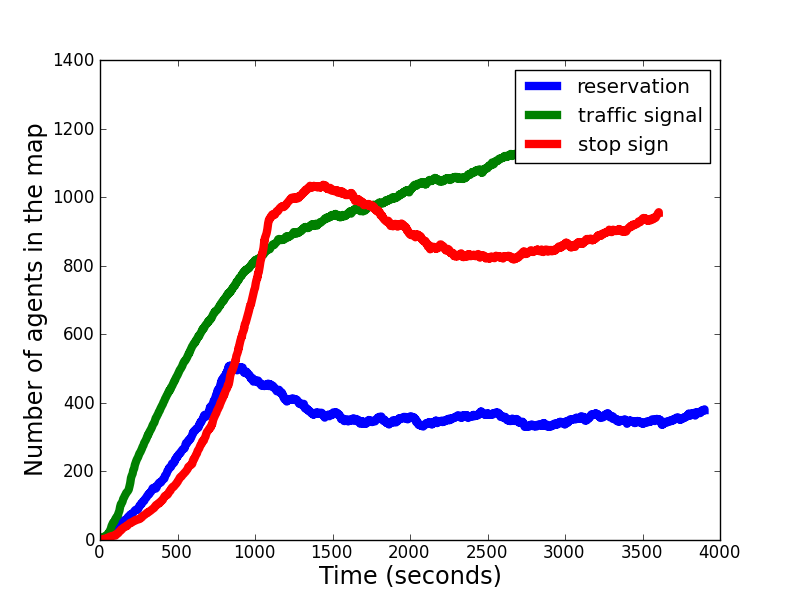
\includegraphics[width=\linewidth]{agent_cnt_atx.png}
  \caption{Autonomous reservations outperform stop signs, and traffic signal
           gridlocked.}
  \label{fig:agent_cnt}
  \vspace{-10pt}
\end{figure}

The number of agents changes because the continuous generator introduces a new
agent every second. This count reaches a steady state when the generator
introduces an agent at the same rate as older agents finish their route. Figure
\ref{fig:agent_cnt} reveals that autonomous reservations let agents reach their
destination twice as quickly as the competition, with a steady-state of about
400 agents. The count for traffic signals continues to increase because gridlock
occurred in one segment of the map, causing agents to not finish their route.
Unexpected starvation was also observed: although the signals cycle through
turns regularly, agents cannot proceed when the previous cycle caused a
destination lane to fill and become blocked.

Each policy has its trade-offs in terms of performance and physical hardware
cost, suggesting a mixed approach, perhaps with intersection policies adapting
as traffic conditions shift. Researchers could conduct this experiment and many
others without needing to understand most of AORTA's code-base. The largest
intersection policy, traffic signals with the flooding heuristic for timing
assignment, is only 400 lines of Scala.

%%%%%%%%%%%%%%%%%%%%%%%%%%%%%%%%%%%%%%%%%%%%%%%%%%%%%%%%%%%%%%%%%%%%%%%%%%%%%%%%

\section{CONCLUSION}
\label{sec:conclusion}

This paper has presented AORTA, a new city-scale traffic simulation framework
that focuses on ease-of-use and policy configurability. In conjunction with Open
Street Maps, AORTA allows researchers to repeat an experiment in any number of
places with minimal effort. Future work will exploit the flexible infrastructure
of interactions between agent behaviors and intersections by exploring dynamic
replanning and adaptable signal timings. On top of these structures,
applications could experiment with dynamic contra-flow \cite{ITSC11-hausknecht}
or intelligent routing that avoids stopping. There will also be an effort to
improve AORTA as a framework by including a lane-changing model and preventing
gridlock. \commentm{Perhaps mention concurency plans (with TACC) to simulate
arbitrarily large maps?}

AORTA's map construction process, although flexible, is fraught with heuristics,
motivating proposed changes to OSM. Road type annotations imprecisely estimate
the number of lanes and typical speed limits, resulting in incorrect graphs.
Guessing the turns at each intersection makes common road features like right
turn-only lanes and shared center left turn lanes hard to detect. There are many
circumstances where AORTA simulates one intersection as several in close
proximity because roads do not geometrically line up, but semantically they do.
If OSM could encode this, the performance of intersection policies such as
traffic signals would vastly improve in those regions. Other simulators have
identified similar issues before \cite{Krajzewicz_Hertkorn_Ringel_Wagner_2005}.

\commentd{Er, so how do I finally end this?}
\commentm{We still have a bit of passive voice.  How much is acceptable?  I think
	it sounds fine, but I imagine an English professor may disagree.}

\addtolength{\textheight}{-12cm}  % This command serves to balance the column lengths
                                  % on the last page of the document manually. It shortens
                                  % the textheight of the last page by a suitable amount.
                                  % This command does not take effect until the next page
                                  % so it should come on the page before the last. Make
                                  % sure that you do not shorten the textheight too much.

%%%%%%%%%%%%%%%%%%%%%%%%%%%%%%%%%%%%%%%%%%%%%%%%%%%%%%%%%%%%%%%%%%%%%%%%%%%%%%%%

\section*{ACKNOWLEDGMENTS}

The authors would like to thank Dr. Michael Quinlan for his support during the
seminal stages of AORTA and all OpenStreetMap contributers for providing free
maps.

%%%%%%%%%%%%%%%%%%%%%%%%%%%%%%%%%%%%%%%%%%%%%%%%%%%%%%%%%%%%%%%%%%%%%%%%%%%%%%%%

% They're sorted by order of citation, not alphabetically. IEEEtran.bst confirms
% this is the correct "numerical citation style."
\bibliographystyle{IEEEtran}
\bibliography{root}

\end{document}
